\PassOptionsToPackage{dvipsnames}{xcolor}
\documentclass[
  20pt,
  a0paper,
  portrait,
  margin=0mm,
  innermargin=15mm,
  blockverticalspace=0mm,
  colspace=0mm,
  subcolspace=0mm
]{tikzposter}

% setting page parameters of the poster
\geometry{paperwidth=33in,paperheight=46.7in}

% for includegraphics command
\usepackage{graphicx}

\usepackage{amsmath, amssymb}
\usepackage{csquotes}

% 'ul' (underline) command that allows line break 
\usepackage{soul} 

% for reduced spacing in references
\usepackage{setspace}

% defining own color in HTML (hex) scheme
\definecolor{mygreen}{HTML}{666633}

% multiple affiliations
\usepackage{authblk}
% setting font and color of authors block
\renewcommand\Authfont{\LARGE \color{white!80!orange}}
% setting font and color of affiliation block
\renewcommand\Affilfont{\Large\color{white!70!mygreen}}

% modern font package
\renewcommand*{\familydefault}{\sfdefault}% Let's have a sans serif font

\usepackage{tikz}
\usetikzlibrary{shapes.geometric, arrows, positioning, decorations.markings}
\usetikzlibrary{fit}
\usepackage{microtype}
\usepackage{framed}
\usetikzlibrary{decorations.pathmorphing,calc,backgrounds}

\newcommand{\mf}{\mathbf}
\newcommand{\lb}{\left(}
\newcommand{\rb}{\right)}
\newcommand{\lsq}{\left[}
\newcommand{\rsq}{\right]}

\newcommand{\kb}{k_\textup{B}}

\newcommand{\intty}{\int\limits_{-\infty}^{+\infty}}

\newcommand{\bbG}{\mathbb{G}}
\newcommand{\bbI}{\mathbb{I}}

\newcommand{\vpravo}{\hspace{1.5cm}}
\newcommand{\vverh}{\vspace*{-0.05cm}}
\newcommand{\vniz}{\vspace{0.05cm}}
% for references:
\newcommand{\hormove}{\par\hangindent 10mm}

\makeatletter
\def\TP@titlegraphictotitledistance{1cm}
\settitle{\centering \color{titlefgcolor} \vbox{\@titlegraphic \\ [\TP@titlegraphictotitledistance] \bfseries \fontsize{1.75cm}{1.3cm} \selectfont \@title \par} \vspace*{1em} {\fontsize{1.4cm}{1cm}\selectfont \@author \par}} 
\makeatother

\title{\parbox{\linewidth}{ \centering Classical trajectory simulation of the CO$_2$ collision-induced band profile in the far IR spectral range}} 

\author[1, 2]{\underline{Daniil N. Chistikov}}
\author[1]{\underline{Artem A. Finenko}} 
\author[3]{Yulia N. Kalugina}
\author[1, 2]{\underline{Sergei E. Lokshtanov}}
\author[1]{Sergey V. Petrov}
\author[2]{\underline{Andrey A. Vigasin}}

\affil[1]{Department of Chemistry, Lomonosov Moscow State University, GSP-1, Leninskie Gory 1-3, Moscow, 119991, Russia}
\affil[2]{Obukhov Institute of Atmospheric Physics Rus.\,Acad.\,Sci., Pyzhevsky per. 3, Moscow, 119017, Russia}
\affil[3]{Department of Optics and Spectroscopy, Tomsk State University, Lenin av. 36, Tomsk, 634050, Russia}

\usetheme{Simple}

\usetitlestyle[width = \linewidth, roundedcorners=5, linewidth=2pt,titletoblockverticalspace=0mm]{Default}
\usebackgroundstyle{Empty}

% this is size of text for References block
\newcommand{\SIZEOFTEXTREFERENCES}{\small}
% this regulates the size of text
\newcommand{\SIZEOFTEXT}{\normalsize}
% this regulates the size of formulae
\newcommand{\SIZEOFFORMULAE}{\fontsize{20}{16}}

\begin{document}

\maketitle

\begin{columns}
\column{0.4}
\block[titleoffsety=46cm, bodyoffsety=47.0cm]{Introduction}{
\SIZEOFTEXT
\SIZEOFFORMULAE{
    \vpravo There is a growing demand to improve existing methods of collision-induced absorption (CIA) spectra simulation [1]. From the one hand, the impetus to refine presently available theories is due to anticipation of future observations concerning a multitude of exoplanetary atmospheres. From the other hand, there is a remarkable progress in computer facilities that opens access to unprecedented computational performance. \par
    \vpravo The use of computationally heavy pure quantum [2] and molecular dynamics [3, 4] methods of CIA simulation is still infrequent and can hardly satisfy near future practical requirements in terms of variety of molecular constituents and range of temperature. In contrast, the method based on consideration of classical trajectories seems to have good perspective for extensive CIA simulation. Recent analysis [5] of the classical dynamics in laboratory frame of reference permitted satisfactory simulation of the CO$_2-$Rg (Rg = Ar, Xe) rototranslational CIA band profiles. \par 
    \vpravo An alternative trajectory based approach is being developed in our research group. Salient features and some preliminary results of it were recently reported elsewhere [6]. Excellent agreement was demonstrated among our calculated trajectory based rototranslational profiles in N$_2-$N$_2$ and those computed quantum mechanically in [2] or obtained experimentally (see [1] and references therein). We use body-fixed frame in which classical dynamics of a collision as well as quantum chemical electronic energy (PES) and induced dipole (IDS) surfaces are rigorously examined. Present paper shows results concerning CO$_2-$Ar and CO$_2-$CO$_2$ systems. 
}}

\block[titleoffsety=1cm, bodyoffsety=2cm]{Trajectory-based CIA spectra simulation}{
    \SIZEOFTEXT
    \vspace{19.5cm}
    \hspace{5cm}
    \begin{tikzpicture}
        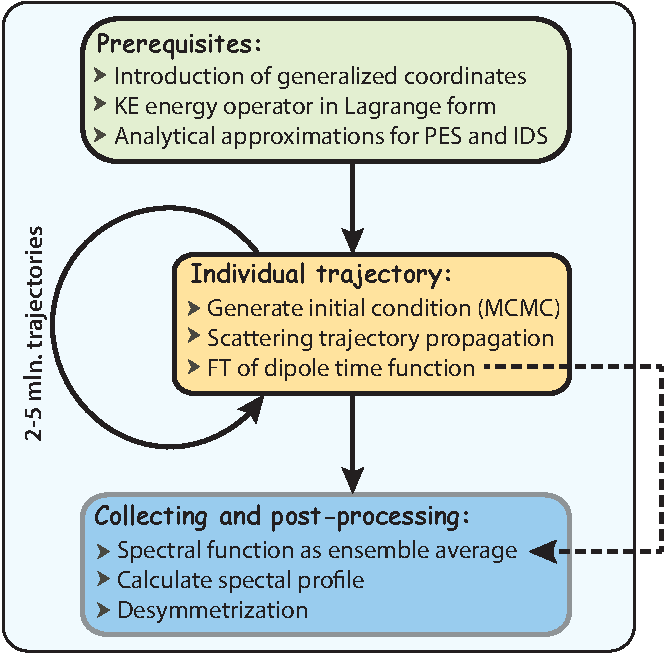
\includegraphics[width=0.6\linewidth]{./pictures/other/scheme-crop.pdf}
    \end{tikzpicture}

    \vspace{0.5cm}
    \vpravo Absorption coefficient $\alpha$ normalized to the product of densities is known to be written as
    \begin{gather}
        \frac{\alpha(\nu, T)}{\rho_1 \rho_2} = \frac{ (2\pi)^2 N_L^2}{3 \hbar} \nu \lsq 1 - \exp \lb -\frac{h c \nu}{\kb T} \rb \rsq V J(\nu, T). \notag
    \end{gather}
    %
    Classical spectral function $J_\text{class}(\nu, T)$ can be found as Fourier transform of the dipole autocorrelation function
    \begin{gather}
        J_\text{class}(\nu, T) = \frac{1}{4 \pi \varepsilon_0} \frac{1}{2 \pi} \intty \langle \mf{d}(0) \cdot \mf{d}(t) \rangle e^{-2 \pi i c \nu t} dt. \notag
    \end{gather}

    As a result of the change of variables that greatly improves the convergence properties of the integral for the free states, we obtained the following expression for classical spectral function
    \begin{gather}
        J_\text{class}(\nu, T) = \frac{1}{4 \pi \varepsilon_0} \frac{1}{2 \pi \Gamma_0} \idotsint \frac{p_R}{\mu} dp_R \exp \lb -\frac{H}{\kb T} \rb d \mf{q}^\prime d\mf{p}^\prime \, \Bigg\vert \intty \mf{d}(t; \mf{q}^\prime, p_R, \mf{p}^\prime) e^{-2 \pi i c \nu t} dt \Bigg\vert^2. \notag
    \end{gather}

    Here $\mu$ is the reduced mass of a molecule pair, $\displaystyle \Gamma_0 = \idotsint \exp \lb -\frac{H}{\kb T} \rb d\mf{q} \, d\mf{p}$ is the normalization factor, $d\mf{q}^\prime$ relates to angular degrees of freedom of each of the monomers and the complex as a whole. 

    \begin{minipage}{0.5\linewidth}
        \begin{tikzfigure}
            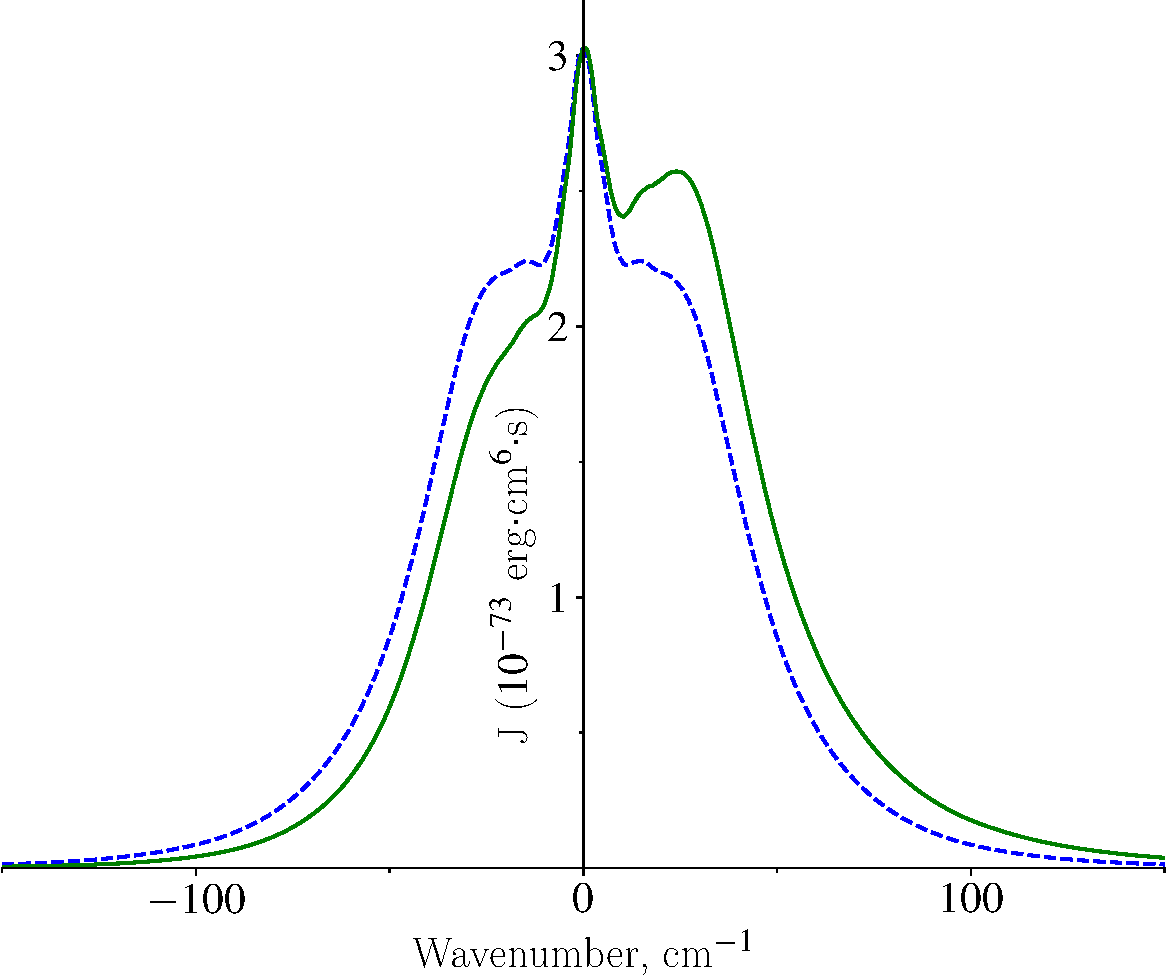
\includegraphics[width=\linewidth]{./pictures/co2co2_spectral_function-crop.pdf}
        \end{tikzfigure}
    \end{minipage}
    \begin{minipage}{0.5\linewidth}
        Simple procedure to account for quantum interaction with EM field:
        \begin{gather}
            J(\nu) = \exp \lb \frac{h c \nu}{\kb T} \rb J_\textup{class}(\nu) \notag
        \end{gather}
        Desymmetrized spectral function satisfies quantum \enquote{detailed balance} principle:
        \begin{gather}
            J(-\nu) = \exp \lb \frac{h c \nu}{\kb T} \rb J(\nu) \notag
        \end{gather}
    \end{minipage}
}

\block[titleoffsety=1cm, bodyoffsety=2cm]{Spectral moments}{
    \SIZEOFTEXT

    \vpravo Spectral moments are integral values, which are widely used to characterise CIA spectra. The use of spectral moments is justified by the possibility to represent them either in terms of integrals over experimentally measured spectral profiles or in terms of Boltzmann weighted functions of induced dipole. \par 
    
    \hspace{6cm} \textbf{Calculation of spectral moments as phase space integrals}
    \begin{gather}
        M_0 = \frac{ \int \mf{d}^2 \exp \lsq -H(\mf{q}, \mf{p}, \mf{J}) / \kb T \rsq d\mf{q} \, d\mf{p} \, d\mf{J}}{\int \exp \lsq -H(\mf{q}, \mf{p}, \mf{J}) / \kb T \rsq d\mf{q} \, d\mf{p} \, d\mf{J}} \qquad 
        M_2 = \frac{ \int \mf{\dot{d}}^2 \exp \lsq -H(\mf{q}, \mf{p}, \mf{J}) / \kb T \rsq d\mf{q} \, d\mf{p} \, d\mf{J}}{\int \exp \lsq -H(\mf{q}, \mf{p}, \mf{J}) / \kb T \rsq d\mf{q} \, d\mf{p} \, d\mf{J}} \notag 
    \end{gather}

    \hspace{6cm} \textbf{Calculation of spectral moments from spectral profile}
    \begin{gather}
        M_0 = 2 \int\limits_0^\infty \lsq 1 - \exp \lb -\frac{h c \nu}{\kb T} \rb \rsq^{-1} \frac{\alpha(\nu)}{\nu} \, d\nu \qquad  
        M_2 = 2 \int\limits_0^\infty \lsq 1 - \exp \lb -\frac{h c \nu}{\kb T} \rb \rsq^{-1} \nu \, \alpha(\nu) \, d\nu \notag 
    \end{gather}

}

\block[titleoffsety=1cm, bodyoffsety=1cm]{Ab initio PES and IDS computation}{
    \SIZEOFTEXT
   
    \begin{minipage}{0.5\linewidth}
        \vspace{11cm}
        \begin{tikzpicture}
            \hspace*{-1cm}
            \includegraphics[width=1.1\linewidth]{./pictures/other/co2co2_potential-trim.png}
        \end{tikzpicture}
    \end{minipage}
    \begin{minipage}{0.5\linewidth}
        \vspace*{-2cm}
        \begin{itemize}
            \item CO$_2-$Ar PES and IDS: CCSD(T)/\textit{aug}-cc-pVQZ and CCSD(T)/\textit{aug}-cc-pVTZ, both supplemented with midbond functions 
            \item CO$_2-$CO$_2$ PES and IDS: CCSD(T)-F12/\text{aug}-cc-pVTZ supplemented with midbond functions
            \item BSSE correction
            \item PES and IDS fit using the basis of spherical functions and cubic splines 
         \end{itemize}
    \end{minipage}

}

\iffalse
\block[titleoffsety=1cm, bodyoffsety=1cm]{Discussion}{
    \SIZEOFTEXT

    Currently in our calculation we disregard the following contributions and factors
    \begin{itemize}
        \setlength\itemsep{0.2em}
        \item quadrupole absorption in an individual CO$_2$ molecule: varies linearly against pure gas pressure and produces different bandshape
        \item absorption belonging to isotopically substituted CO$_2$ molecule,
        \item true bound dimer absorption: amounts up to 10\% of total intensity at near room temperature and is more pronounced at lower temperatures,
        \item fraction of CO$_2$ molecules occupies (010) bending state: expected to increase at elevated temperature, however, the regular mismatch between calculated and measured spectra is not currently observed.
    \end{itemize}
}
\fi

\column{0.6}
\block[titleoffsety=46cm, bodyoffsety=48.5cm]{CO$_2-$CO$_2$ rototranslational band}{
    \SIZEOFTEXT
    \begin{tikzfigure}
        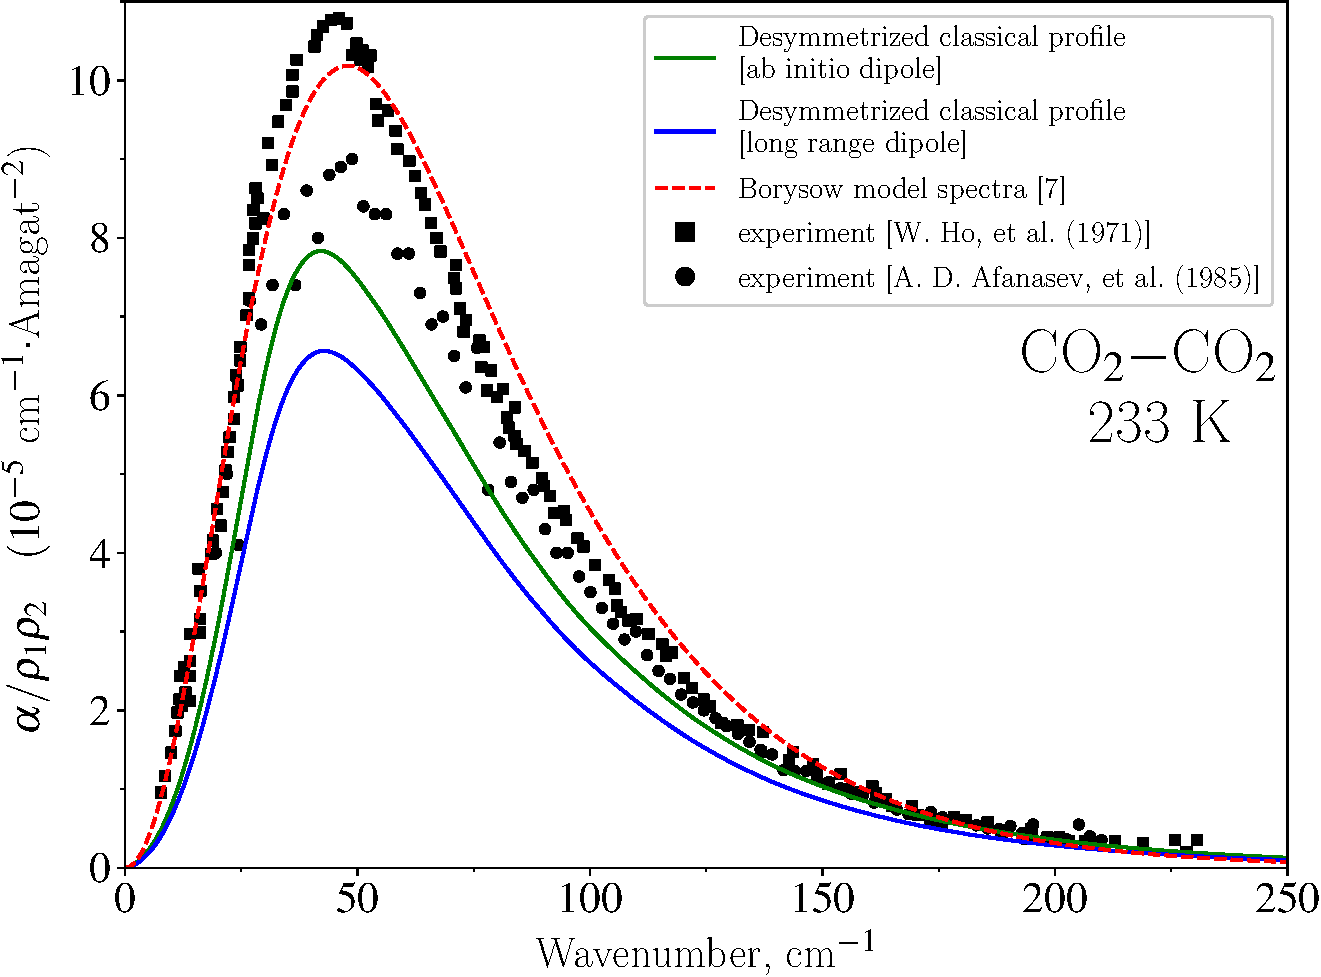
\includegraphics[width=0.49\linewidth]{./pictures/CO2-CO2-233K-legend-crop.pdf}
        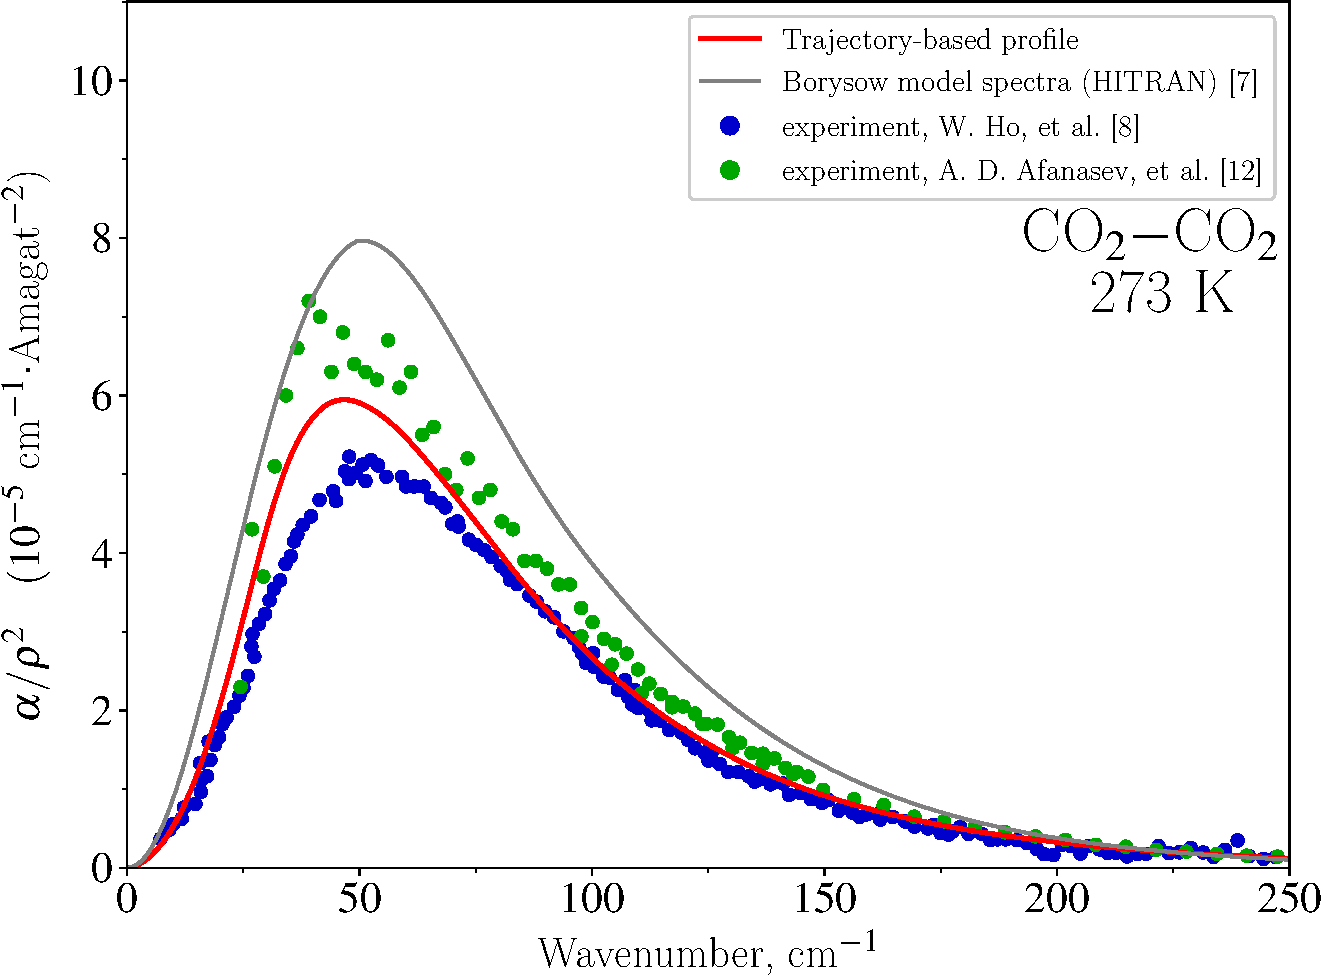
\includegraphics[width=0.49\linewidth]{./pictures/CO2-CO2-273K-legend-crop.pdf} \\[1em]
        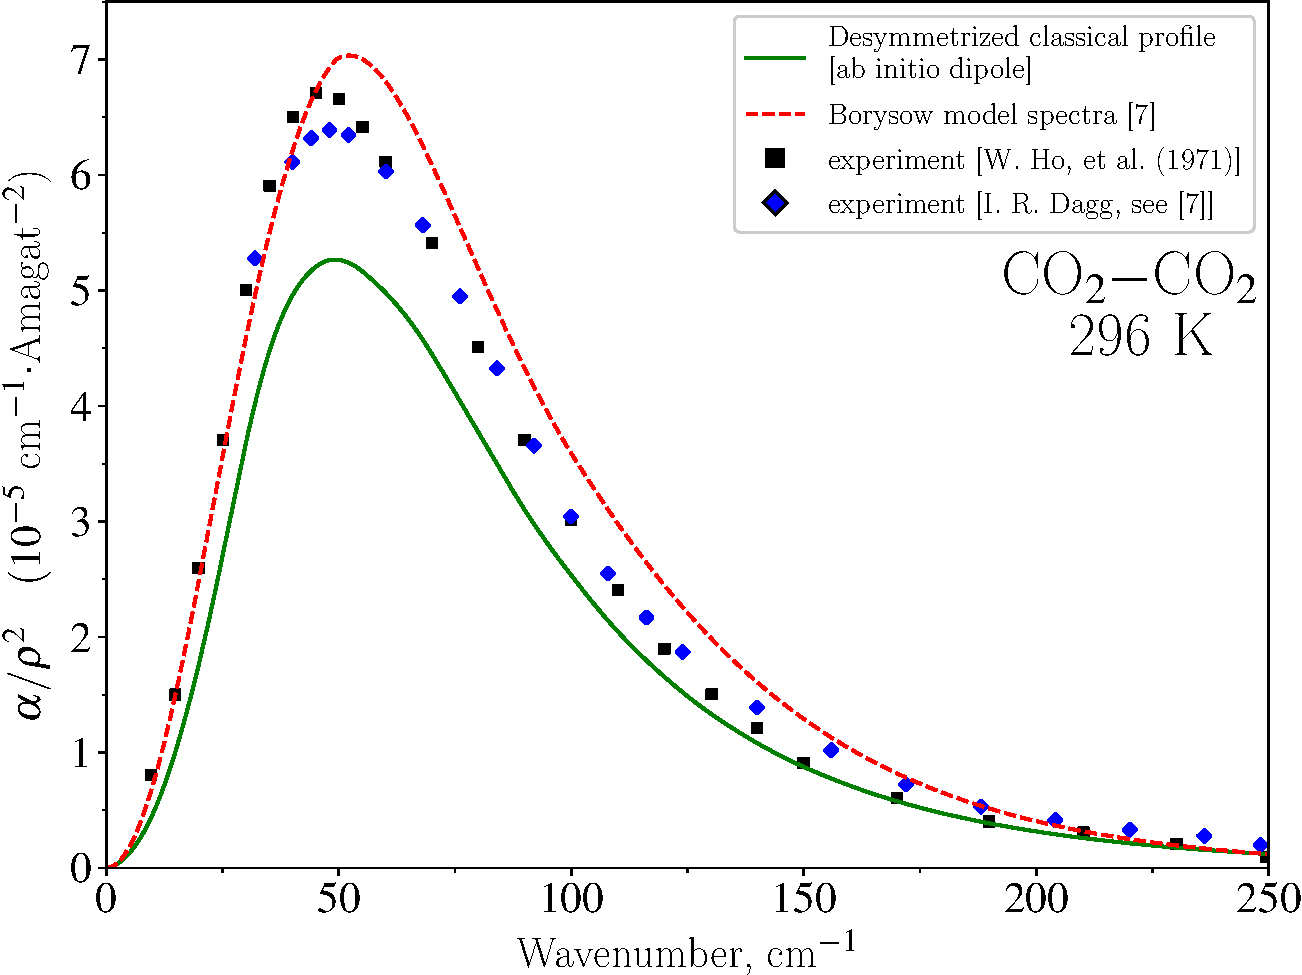
\includegraphics[width=0.49\linewidth]{./pictures/CO2-CO2-296K-legend-crop.pdf}
        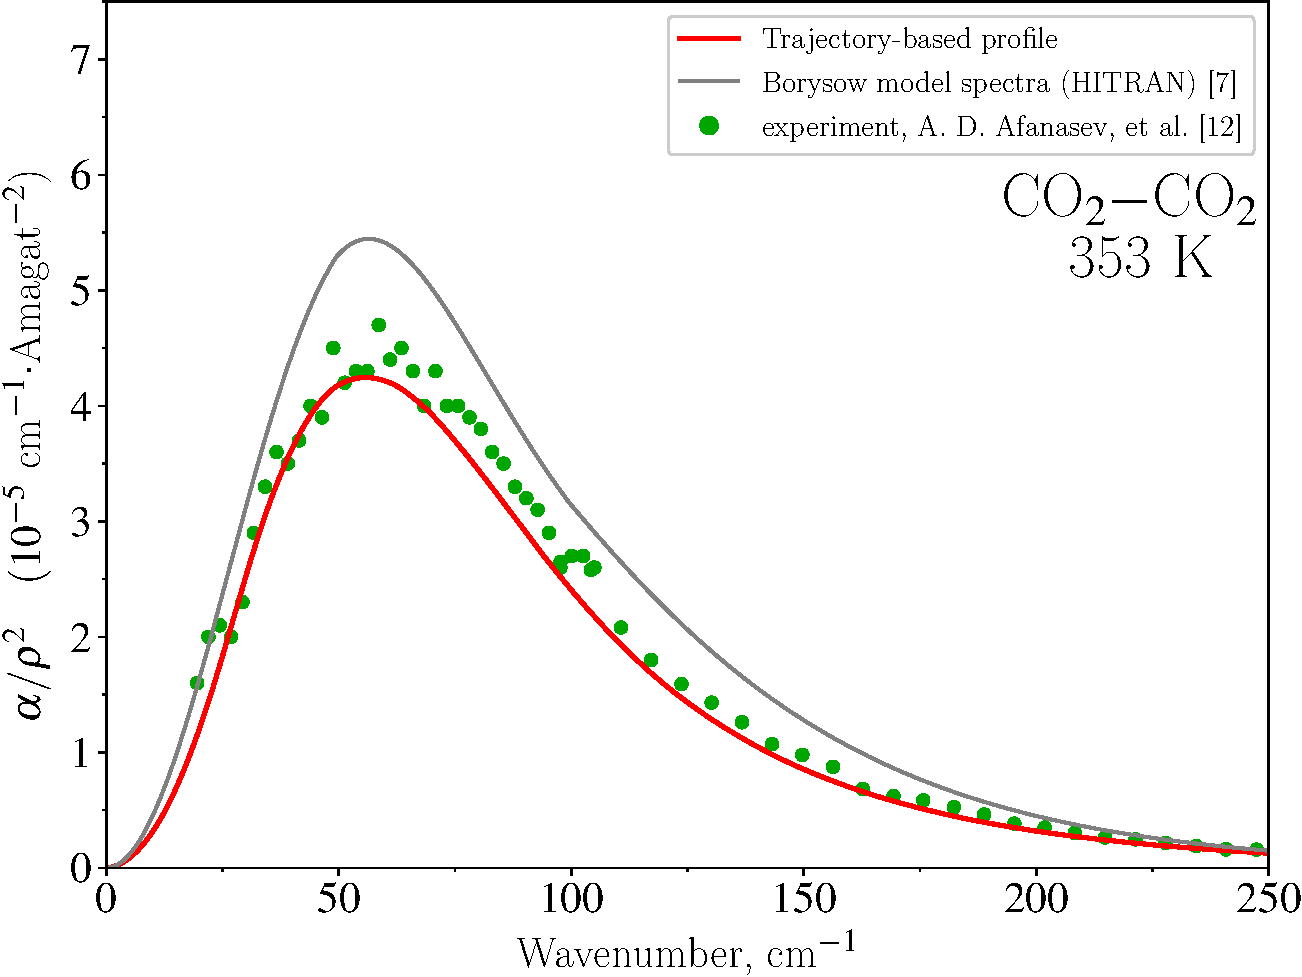
\includegraphics[width=0.49\linewidth]{./pictures/CO2-CO2-353K-legend-crop.pdf}
    \end{tikzfigure}
}

\block[titleoffsety=2.0cm, bodyoffsety=4.0cm]{CO$_2-$Ar rototranslational band}{
    \SIZEOFTEXT
    \begin{tikzfigure}
        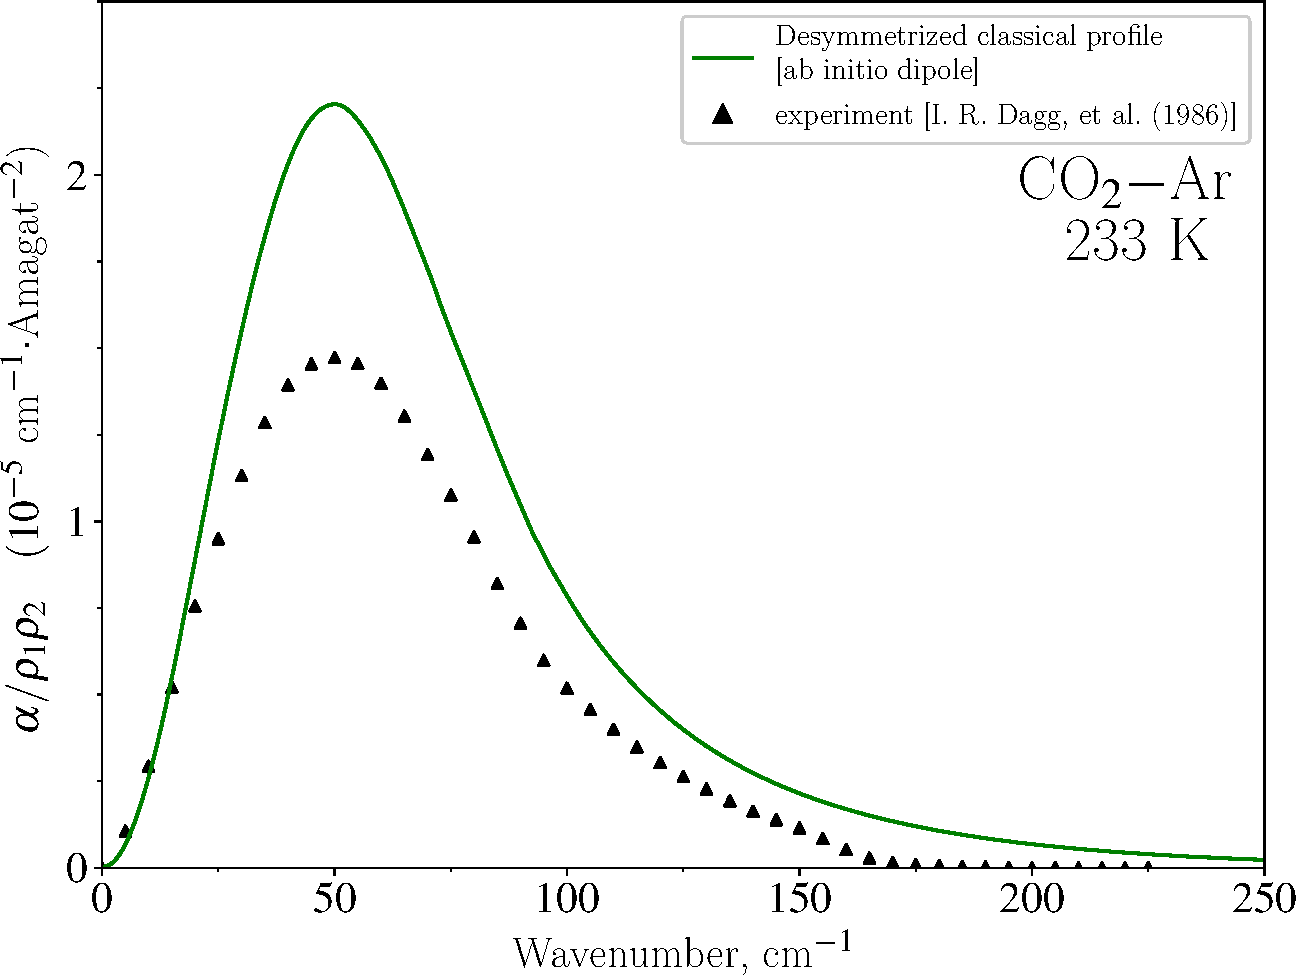
\includegraphics[width=0.49\linewidth]{./pictures/CO2-AR-233K-legend-crop.pdf}
        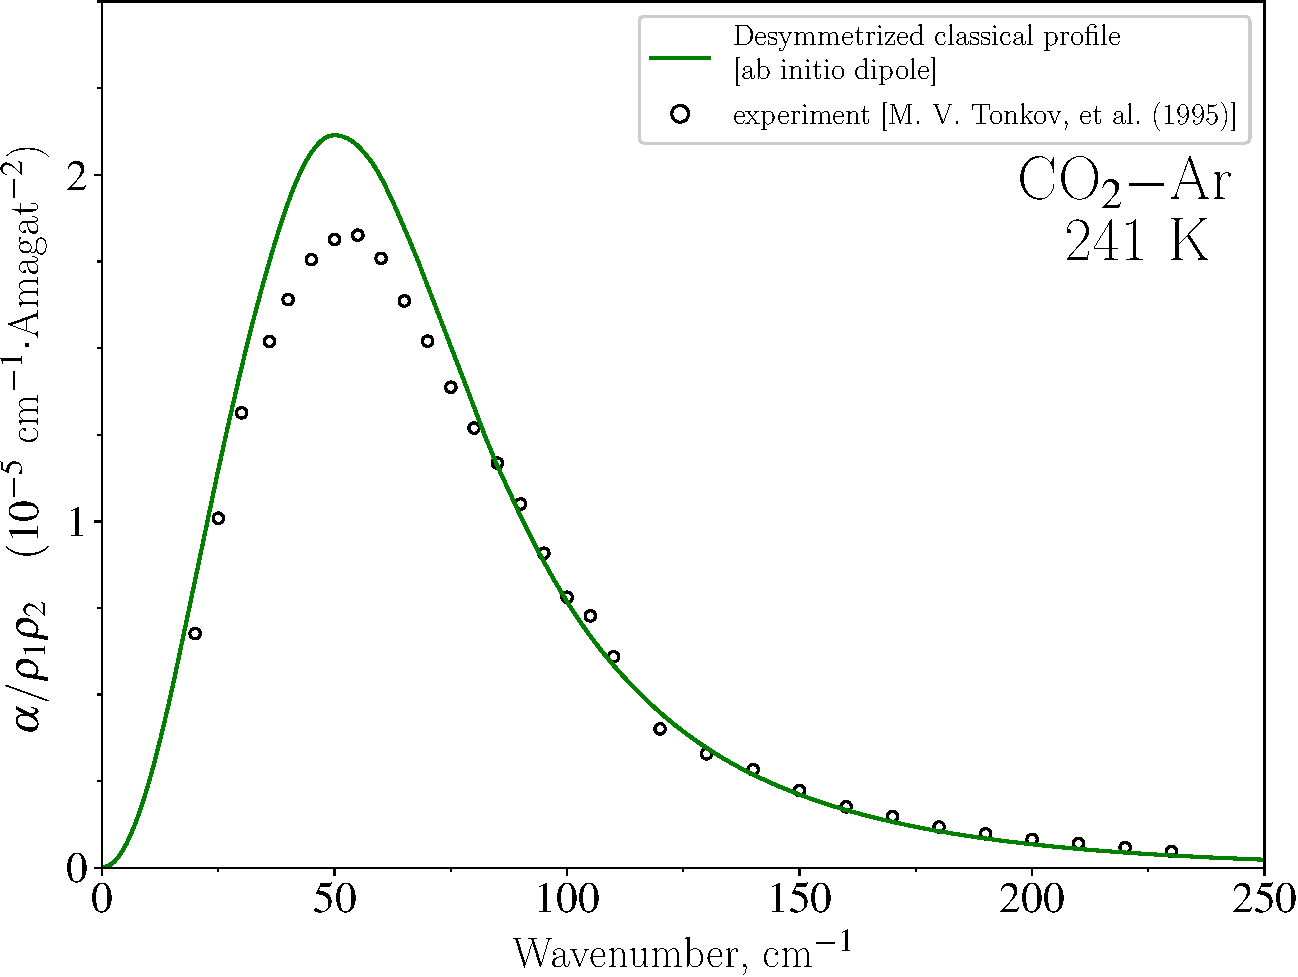
\includegraphics[width=0.49\linewidth]{./pictures/CO2-AR-241K-legend-crop.pdf}
        %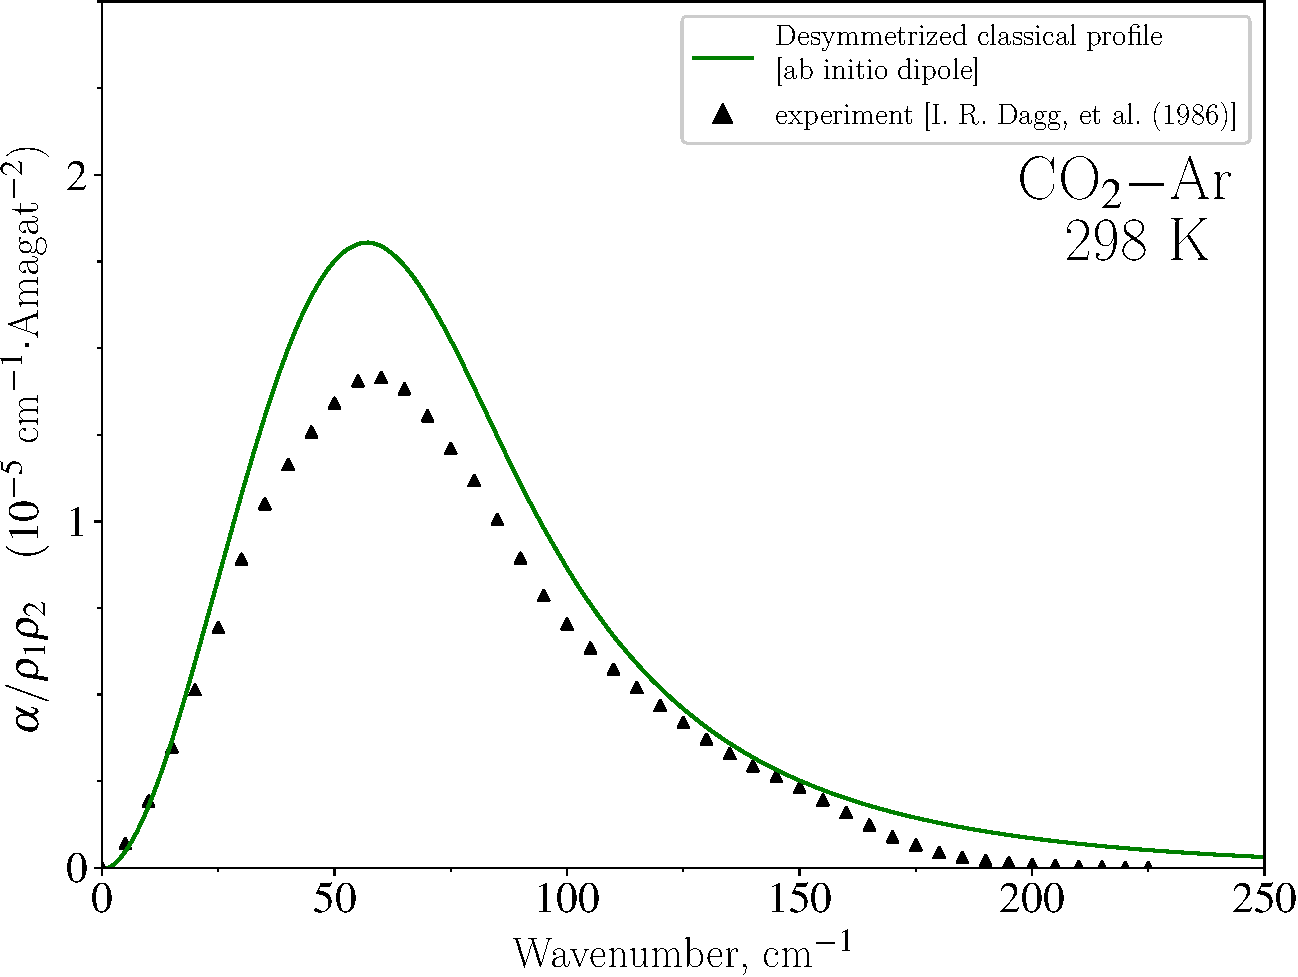
\includegraphics[width=0.49\linewidth]{./pictures/CO2-AR-298K-legend-crop.pdf}
        %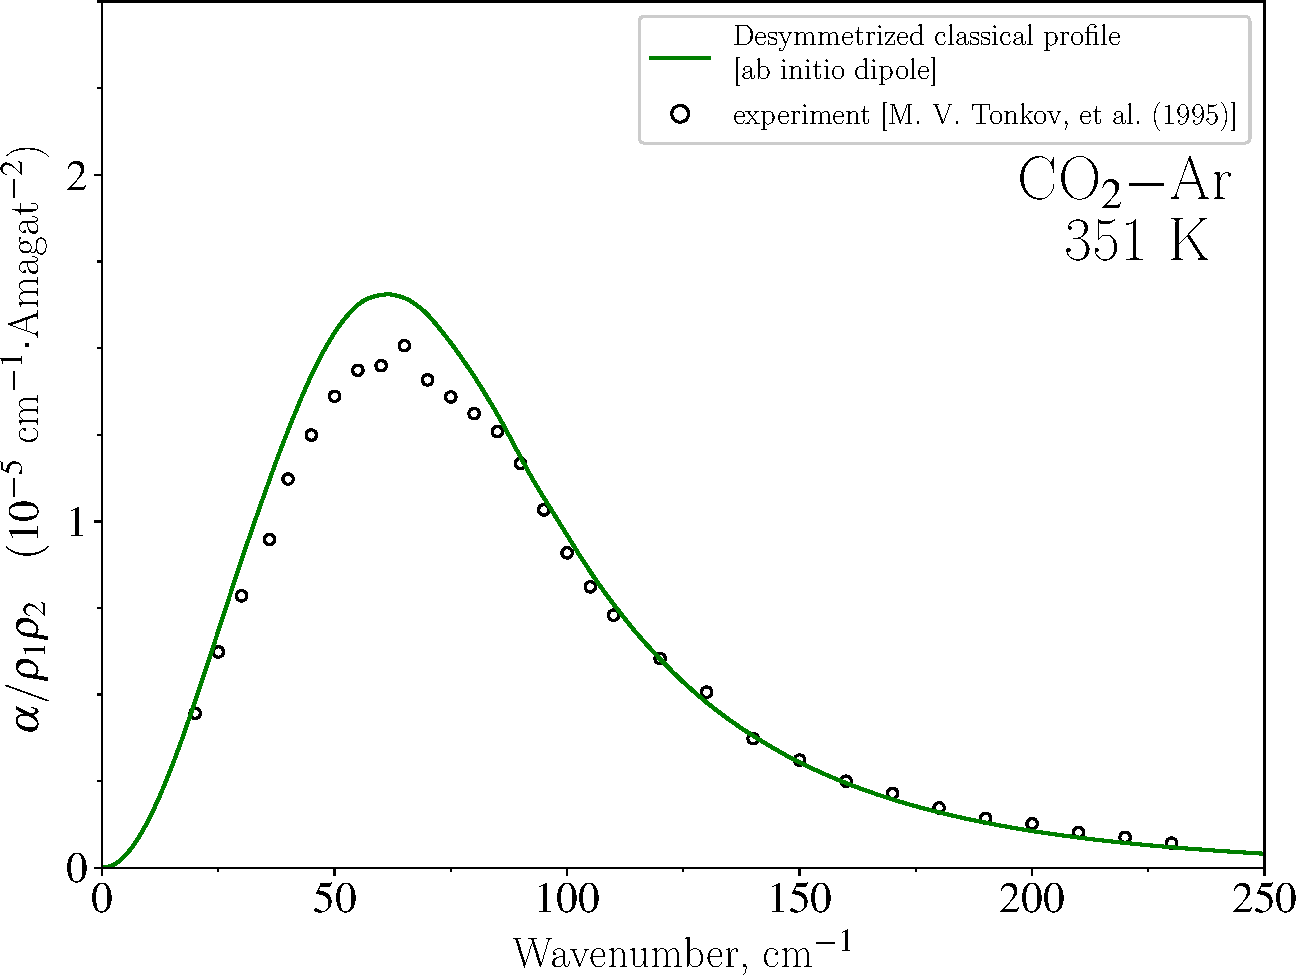
\includegraphics[width=0.49\linewidth]{./pictures/CO2-AR-351K-legend-crop.pdf}
    \end{tikzfigure}
}

\block[titleoffsety=1.5cm, bodyoffsety=4.0cm]{Experimental vs.\! calculated CIA intensities}{
    \begin{tikzfigure}
        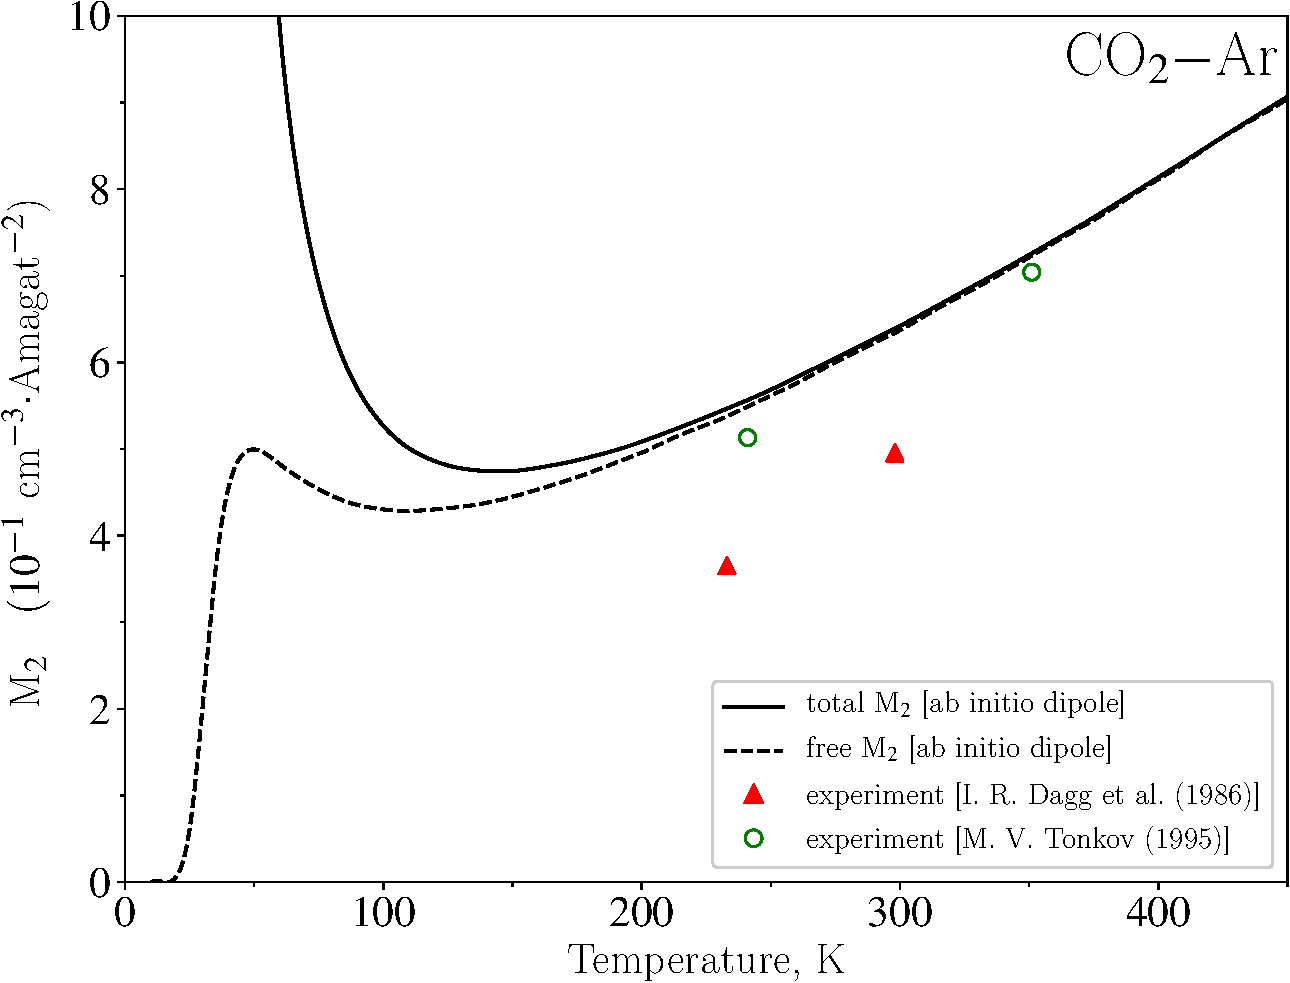
\includegraphics[width=0.40\linewidth]{./pictures/CO2-AR-second-moment-legend-crop.pdf}%
        \hspace{4cm}%
        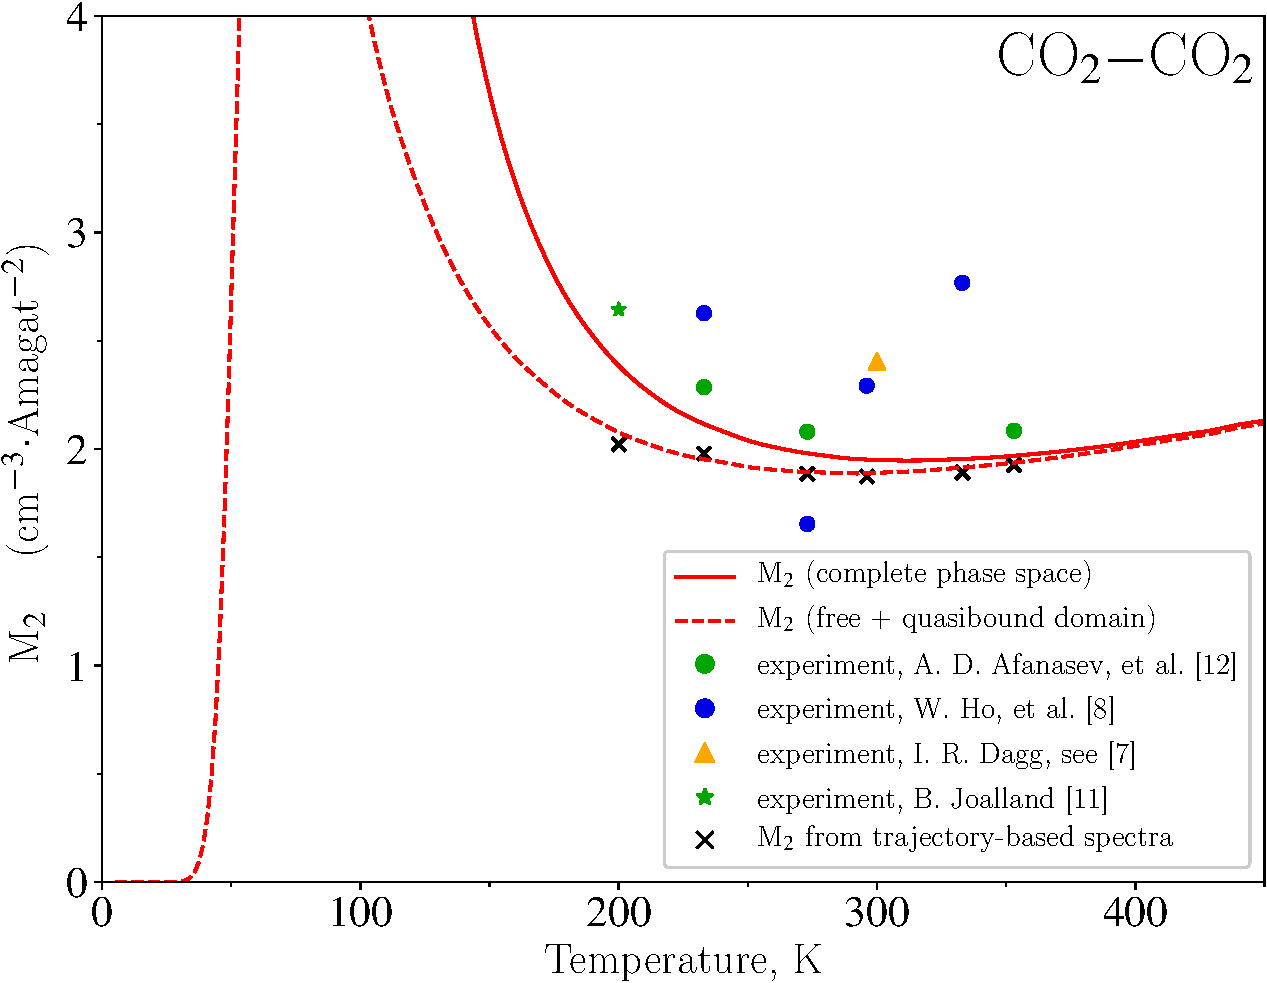
\includegraphics[width=0.40\linewidth]{./pictures/CO2-CO2-second-moment-legend-crop.pdf}
    \end{tikzfigure}
}

\block[titleoffsety=2cm, bodyoffsety=3.0cm]{Conclusions}{
    \SIZEOFTEXT
    \vpravo The results reported here show encouraging perspective for our trajectory based method to be employed in extensive CIA simulation. To the best of our knowledge, trajectory based calculation of CIA spectra for various pairs of linear molecules is performed for the first time. Moreover, we extended calculations to CO$_2-$CO$_2$ pair which is known to possess strong anisotropy of intermolecular interaction. We admit that ensemble of available experimental data for CO$_2-$CO$_2$ is yet not perfectly reproduced by our trajectory based calculations. Nevertheless, overall agreement is quite reasonable bearing in mind an appreciable uncertainty, which characteristic to experimental data issuing from different laboratories. Moreover, in contrast to some series of experimental data our spectra vary regurarly as a function of temperature. These calculated variations are strongly supported by our independent computations of the zeroth and the second spectral moments as integrals over phase space. 
}

\block[titleoffsety=1cm, bodyoffsety=2.5cm]{Acknowledgements}{
    \SIZEOFTEXT
    The authors gratefully acknowledge invaluable help from R. Wordsworth in the use of computer facility at Harvard university. The work was supported in part by RFBR Grants 18-05-00119 and 18-55-16006 as well as Presidium of RAS Program 28.
}

\block[titleoffsety=1.0cm, bodyoffsety=2.5cm]{References}{
\SIZEOFTEXTREFERENCES
1. T.\,Karman, I.\,E.\,Gordon, A.\,van der Avoird, \textit{et al}. (2019) \textit{Icarus} 328, 160-175. \\
2. T.\,Karman (2018) \enquote{Collision-induced absorption by oxygen and nitrogen molecules}, PhD thesis, Radboud University. \\
3. J.-M.\,Hartmann, \textit{et al}. (2011) \textit{J. Chem. Phys.} 134 (9), 094316. \\
4. B.\,Bussery-Honvault, and J.-M.\, Hartmann (2014) \textit{J. Chem. Phys.} 140 (5), 054309. \\ 
5. D.\,Oparin, N.\,N.\,Filippov, I,\,M.\,Grigoriev, \textit{et al}. (2017) \textit{J. Quant. Spectr. Radiat. Transf.} 196, 87-93. \\
6. D.\,N.\,Chistikov, A.\,A.\,Finenko, Y.\,N.\,Kalugina, \textit{et al}. (2018) \textit{Classical trajectory simulation of collision-induced absorption spectra}. HRMS, Bilbao, Spain. \\
7. M.\,Gruszka, and A.\,Borysow (1997) \textit{Icarus} 129, 172-177. \\
8. W.\,Ho, G.\,Birnbaum, and A.\,Rosenberg (1971) \textit{J. Chem. Phys.} 55 (3), 1028-1038. \\
9. I.\,R.\,Dagg, A.\,Anderson, S.\,Yan, \textit{et al}. (1986) \textit{Can. J. Phys.} 64 (11), 1475-1481. \\
10. M.\,V.\,Tonkov (1995) In: \textit{Collision- and Interaction-Induced Spectroscopy}. Kluwer AP. \\ 
11. B.\,Joalland, M.\,Goubet, R.\,Georges, \textit{et al}. (2016) \enquote{Far-infrared collision-induced absorption in CO$_2$ at T = $200$ K}. 13th ASA Conference, Reims. \\
12. A.\,D.\,Afanasev, N.\,M.\,Grigorovich, and M. V.\,Tonkov (1985) \textit{Opt. Spectrosc.} 58, 772-774.
}

\end{columns}


\end{document}
